\chapter{Forward and inverse kinematics}

\section{UR5}
Universal Robots (UR1,-3,-5,-10) are multifunctional, flexible robots that can be used for various tasks. 
The number stands for the working load and therefore also the size of the robot. These robots 
are place saving and can be easily reprogrammed for new requirements. \\

ref1 \\

The URs consist out of six rotational joints and seven fixed links. Therefore there are eight different
constellations of joint angles to reach a determined end-effector position. That means that for given joint parameters we can calculate one unique position, but for a given position there are eight different sets of angles. These eight constellations can be described as lefty/righty, up/down and flip/noflip. With lefty/righty we can distinguish between the second joint being on the right or left
side of the imaginary plane going through the origin of the coordinate system of the first joint. This distinction makes sence if the coordinate system of the second joints has an offset according to the coordinate system of the first joint.  Up/down describes the relation between the coordinate systems of the third and the fourth joint. If the fourth joint remains in the same position, the third joint can 
be below or above it. Therefore we distinguish between up and down. Finally flip/noflip describes
the wrist (5th joint) being flipped or not, meaning rotated by $\phi$ or $\phi$ + 180$^\circ$. 

\begin{minipage}{0.64\textwidth}	
		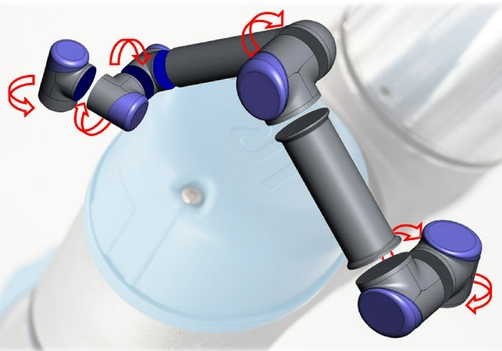
\includegraphics[width=\textwidth]{UR_joints}			
		\captionof{figure}{Joints of the UR, ref2}
\end{minipage}
\begin{minipage}{0.34\textwidth}
		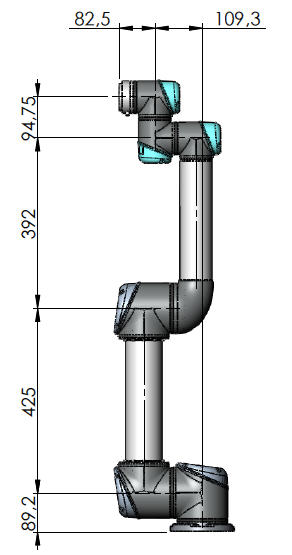
\includegraphics[width=\textwidth]{UR_dimensions}	
		\captionof{figure}{Dimensions of the UR, ref3}		
\end{minipage}

	%\begin{figure}[htbp]
		%\centering 
		%\captionsetup{format=plain}
			%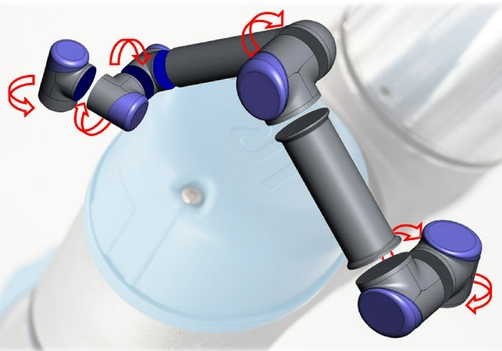
\includegraphics[width=1\textwidth]{UR_joints.jpg}		
				%\caption{Joints of the UR} 
				%\label{URJoints} 
	%\end{figure}

\section{Forward kinematics}
The forward kinematics of this kind of robot can be calculated easily with the Denavit-Hartenberg-procedure if the parameters are known. Denavit-Hartenberg-parameters describe the relation between two coordinate systems with a maximum of four different parameters: two rotation angles 
and two linear translations. These can be fixed or variable. In our case with six joints we have seven coordinate systems and six transfomations. Coordinate system zero is not attached to any of the joints and is used as the reference frame. \\

\section{Backward kinematics}
The backward kinematics has been realised with the algorithm of paper 

ref4 \\
 
Its starting point is the desired pose that we want to move our robot to. 
With this pose and the given Denavit-Hartenberg-parameters we calculate intermediate
poses from which the six angles can be found step by step. Previously calculated angles can furthermore be used to calculate the next ones. Since there are different angles possible to reach the same pose, it is important to name the current angle that is being used to calculate the next one. Lefty/righty, up/down and flip/noflip are current names. In case that one angle has two solutions the current solution exist with its particular name so
that the distinction between different possibilities is made. \\

The implemented algorithm works as follows:

\begin{itemize}
	\item Calculate eight max possible angle configurations that lead to the desired pose 
	\item Check if the pose is possible with the robots dimensions and/or the given maximal joint changes
	\item Calculate the $\pm$ 360$^\circ$-versions of the found angles since the robot might be able 
	to move in the range of $\pm$ 360$^\circ$ and get eight new possibilities
	\item Choose one angle set of the 16 sets with the minimal angle sum with respect to the initial angles
\end{itemize}